\chapter{Related Work}\label{chapter:relatedwork}

\section{Datasets for driver behavior analysis}

As of the time of writing, numerous datasets are available for driver behavior analysis, each with its own specific focus. For instance, \textbf{DR(eye)VE Dataset}\cite{palazzi2018predicting}capturing drivers' gaze patterns in real-world scenarios, includes ego-centric views and car-centric views, which provide data on where drivers look in different driving contexts. \textbf{Naturalistic Driving Study (NDS)}\cite{regan2012naturalistic} contains extensive data collected from naturalistic driving conditions, including in-vehicle driver behavior such as driver movements, eye gaze, and interactions with vehicle controls during different driving scenarios.


In our work, we utilize the \textbf{Drive \& Act} dataset\cite{9009583} as our primary training resource. This dataset includes over twelve hours and 9.6 million frames, capturing individuals engaged in various distractive activities during both manual and automated driving. It is specialized for distinguishing between closely related actions (e.g., opening a bottle vs. closing a bottle) and features a high diversity in action durations and complexities, presenting unique challenges for action recognition models. For instance, brief actions like opening a door from the inside may take less than a second, while prolonged activities such as reading a magazine may last several minutes. This dataset is exceptionally well-suited to our study, as it provides a comprehensive view of driver behavior within the vehicle, with accurately labeled, temporally sequenced annotations for each behavior.


\begin{figure}
    \centering
    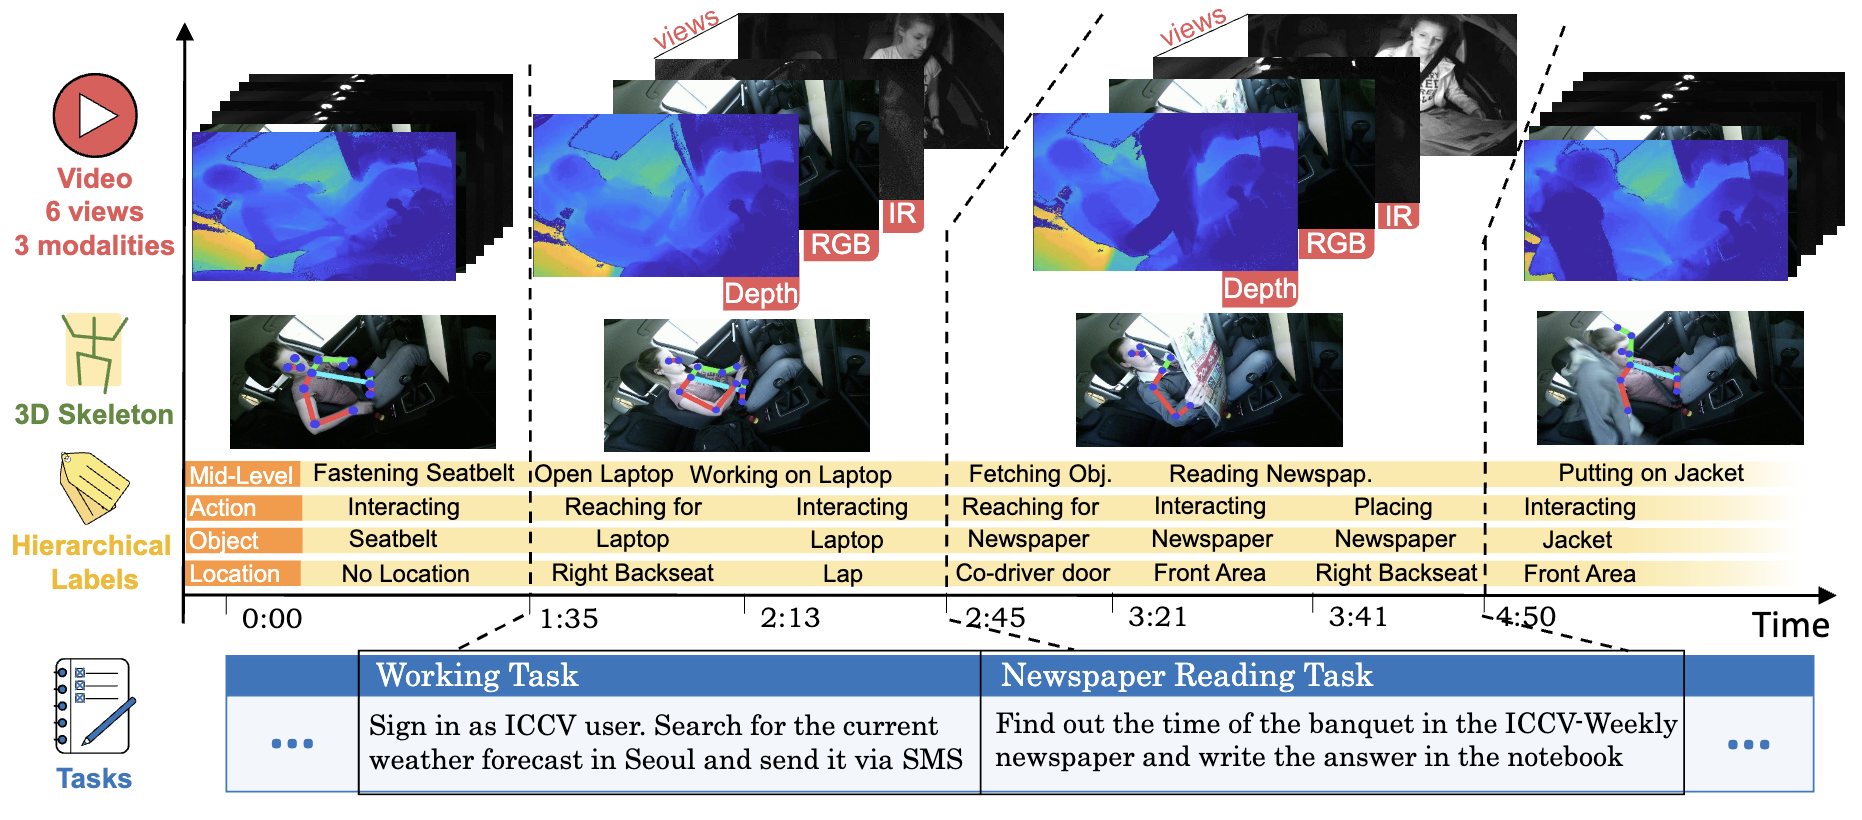
\includegraphics[width=\linewidth]{figures/03_DriveAct.png}
    \caption{Overview of the Drive\&Act dataset for driver behavior recognition. Reproduced from\cite{9009583}}
    \label{fig:DriveAct}
\end{figure}

\section{Dynamic Scene Graph for Video}

As is revealed in chapter\ref{chapter:background}, the most common way to represent the latent information in a video is to use CNNs to directly extract the features of the frames and then use RNNs to model the temporal information. However, this method has its limitations as the excessive high-dimensional abstraction may cause the model to misinterpret human learning intentions; in other words, the black box itself is difficult to interpret. In our work we would like to extract the dynamic scene graph from the video, which is a more intuitive way to represent the video content.

The scene graph is a structured representation of a scene that can clearly express the objects, attributes, and relationships between objects in the scene\cite{9661322}. Accompanied by the development of computer vision technology, simply detecting and recognizing objects in images no longer satisfies the researchers, as they would expect some higher level of understanding and reasoning for image vision tasks. In this way, an intuitive idea comes up about adding up the relationship between the detected objects (See example in figure\ref{fig:SGG}). The earliest research could date back to 2017, when some objects and relations of a given image could be inferred, and a scene graph would be produced as a result\cite{xu2017scene}. Other research like Neural Motifs\cite{zellers2018neural} also shows the possibility of predicting the most frequent relation between object pairs with the given labels and object detections. Later in 2018, videos came into discussion, and both spatial and temporal relations would be concerned in the dynamic graph researchers propose to represent\cite{wang2018videos}. Meanwhile, the accuracy of Scene Graph Detection tasks has significantly improved thanks to the application of unbiased SGG\cite{wang2018videos}, fueled by the \textbf{Detection2} \cite{wu2019detectron2}, a library that contains various state-of-the-art detection and segmentation algorithms. In a nutshell, representing videos as dynamic scene graphs including the detection of objects and the relations in between has been realized in the past years. And our work would utilize such technique and extract our driver-oriented dynamic scene graphs for further learning.

\begin{figure}
    \centering
    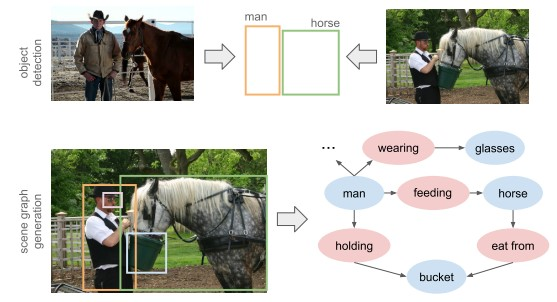
\includegraphics[width=\linewidth]{figures/03_SGG.jpg}
    \caption{Scene Graph Generation by Iterative Message Passing. Reproduced from\cite{tang2020unbiased}}
    \label{fig:SGG}
\end{figure}

\section{Dynamic Link Prediction}

After extracting the dynamic scene graph from the video, the next step involves learning the features between elements to enable behavior prediction. Thus, our primary task can be framed as link prediction within the dynamic scene graph, making the choice of a suitable model essential to the success of our work. Thanks to ~\text{DGB}\cite{poursafaei2022towards}, we have a comprehensive review of existing link prediction models and effective evaluation strategies for assessing their performance. Below, we provide an introduction to each model, along with a theoretical explanation of our final selection.

\subsubsection{JODIE}
Based on the user-item interaction data, JODIE\cite{kumar2019predicting} works as a coupled Recurrent Neural Networks(RNN). The update operator alternatively updates the embedding space of suer and an item at each interaction. And the projection operator learns to estimate the embedding of the user at any time in the future, which is used to predict the next interactions. 

\subsubsection{DyRep}
DyRep\cite{trivedi2018representation} is an inductive deep representation learning framework that learns a set of functions to efficiently produce low-dimensional node embeddings that evolves over time. The model captures all the new edges appears during the time sequence and upates the embeddings of the nodes accordingly in a custom RNN model. The final output provides a solution to the problems of dynamic link prediction and event time prediction.
% probleom: only on +

\subsubsection{TGN}
\textbf{TGN}\cite{rossi2006temporal} is a generic, efficient framework for deep learning on dynamic graphs represented as sequences of timed events. To train the Memory-related modules, the message matrix would begin with a raw message store and is updated based on interactions which have been processed by the model in the past, which would also propagate to the node embedding as well as the loss function.  TGNs significantly outperform previous approaches while being more computationally efficient.

\subsubsection{CAWN}
Based on temporal random walks, \textbf{CAWs} adopt a novel anonymization strategy that replaces node identities with the hitting counts of the nodes based on a set of sampled walks to keep the method inductive, and simultaneously establish the correlation between motifs. It is specialized in work as automatic retrieval of temporal network motifs to represent network dynamics. Since our dataset has only little similarity with random walking, we didn't take this into consideration at last.

After experience on all the above models, our work finally adapted the model \textbf{JODIE}. This is theoretically plausible because our dataset holds the form of participator-object, which is quiet similar to user-item interaction data in structure. No denying that \textbf{TGN} also has a sophisticated structure, however it require a huge amount of data to train, which is unaffordable for our dataset.